\documentclass[11pt,a4paper]{article}
\usepackage[latin1]{inputenc}
\usepackage[spanish]{babel}
\usepackage{amsmath}
\usepackage{amsfonts}
\usepackage{amssymb}
\usepackage{apacite}
\usepackage{graphicx}
\usepackage[left=2cm,right=2cm,top=2cm,bottom=2cm]{geometry}
\author{Samuel Caleb Martinez Hernandez}
\title{Instalacion de ROS }
\date{13 de Septiembre del 2019\\
Integrantes\\
Martinez Hernandez Samuel Caleb\\
Canales Ochoa Fabian\\
Flores Macias Cesar Fabian\\
Gutierrez Chavez Amaury Efrain\\}
{
\begin{document}
\maketitle
\section{Introduccion }
Antes de entrar en materia, debemos saber que es lo que vamos a instalar, es decir, conocer el material que vamos a instalar en nuestros ordenadores y la razon.

\centering
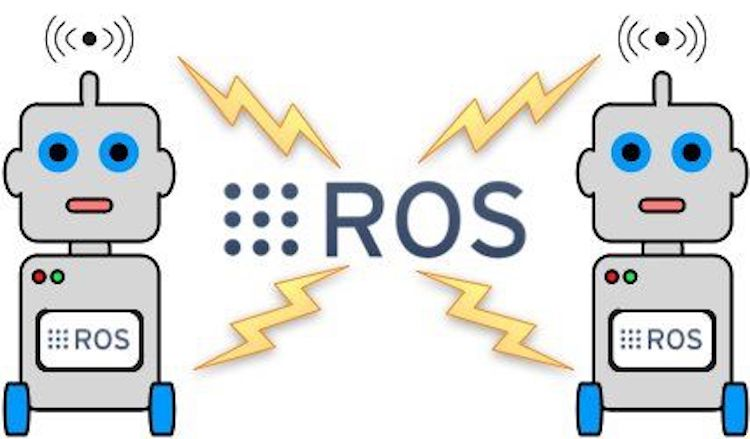
\includegraphics[width=10cm]{EV1/Ros.jpg} 

{
En palabras claras, ROS es un software enfocado en el desarrollo de software para robots. Incluyendo entre sus capacidades la posibilidad de abstraccion de hardware robotico, control de dispositivos de bajo nivel, la implementacion de funcionalidad de uso comun, el paso de mensajes entre procesos y el mantenimiento de paquetes.
}
}

\section{Requisitos}

X  Linux con Ubuntu.

X  Conexion a internet.

X  Al menos 3 GB's de espacio libre.

{
\section{Desarrollo}
Lo mas logico es que cuando se trata de instalar un software, por motivos de seguridad, este se descargase desde la web oficial o autorizada y para nuestra suerte, este software si que la tiene, aquí el link: "http://wiki.ros.org/ROS/Installation".
}
{

\begin{center}
  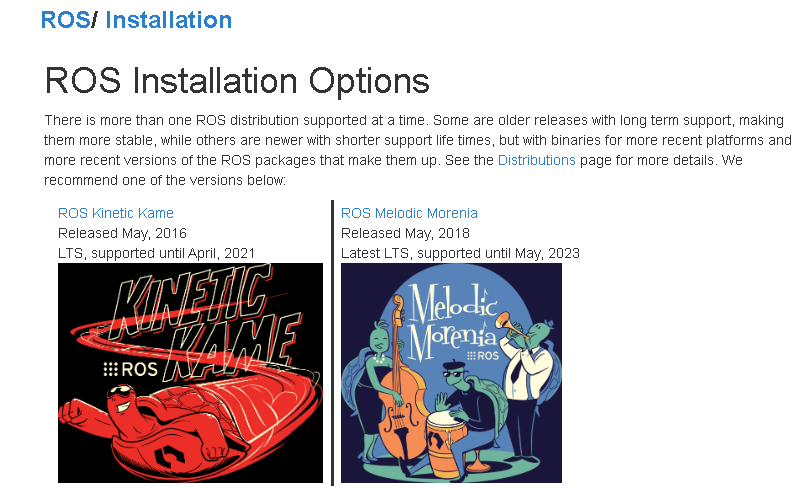
\includegraphics[width=10cm]{EV1/Ros1.png} 
  \end{center}  
}

{
\section{Kinetic o Melodic}

Sea "Melodic" o "Kinetic" ... o amabas, la isntalacion tiende a ser el mismo prosedimiento, por lo que para intalarlo en ubuntu, el proceso es algo distinto, ya que este de hace desde la consola. 

En fin, el link: "http://wiki.ros.org/kinetic/Installation/Ubuntu" nos muestra los comando necesarios para instalar ROS, desde luego, seguiremos uno por uno.
}

{
\section{Sources}

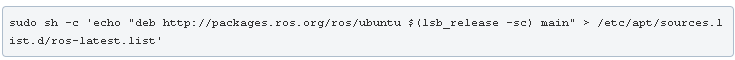
\includegraphics[scale=0.8]{EV1/1.png} 
}

Este comando nos permite el acceso de software a la computadora.

\section{Keys}

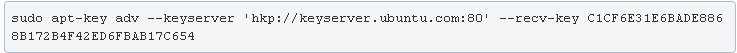
\includegraphics[scale=0.8]{EV1/2.png}

El comando anterior otorga las llaves correspondientes del servidor de la descarga del software. 

\section{Update}

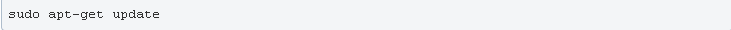
\includegraphics[scale=0.8]{EV1/3.png}

Antes de poder querer isntalar algo apropiadamente, se debe de tener un sistema operativo bien actualizado, para de esta manera poder aprovechar al maximo las capacidades del software en cuestion, en pocas palabras, hay que actualizar de ser posible. 

\section{Instalacion de ROS}

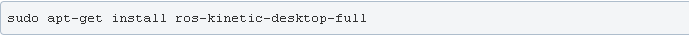
\includegraphics[scale=0.8]{EV1/4.png}

Es decision de cada quien el si se desea descargar la version completa de ROS o las versiones individuales como los paquetes individuales, Ros-Base, entre otras librerias. En esta ocasion se enfocara en la instalacion de la version completa. ( Siendo "apt-cache search ros-kinetic" el que busca paquetes disponibles).

\section{Dependecias de ROS}

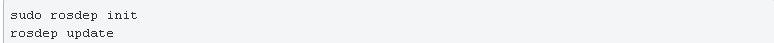
\includegraphics[scale=0.8]{EV1/5.png}

Para empezar a usar ROS es conveniente que se instalen las dependencias que provienen de fuentes oficiales de la pagina, siendo algunos de estos necesarios para ciertos procesos. 

\section{Ambiente de ROS}

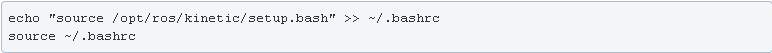
\includegraphics[scale=0.8]{EV1/6.png}

Para terminar, este comando descarga los ambientes en los que trabajara ROS.

\section{Conclusion}
Samuel Caleb:
Como era de esperarse, cuando se trata de una instalacion de software enfocado a robots, es logico que se trate de un proceso bastante estructurado, por asi decirlo, "bien construido", sobre todo por la cantidad de descargas colaterales de las cuales ROS depende, vaya programa toco instalar. \\ 
\\
Cesar Fabian:
El ROS es un programa creado orignalmente para ubuntu,con el cual podremos realizar sinulaciones de movimientos de robots, y poder aseguranos que tendra un movimiento correcto, aunque la instalacion sea bastante compleja solo son pasos a seguir.
\\ \\
Fabian Canales:
en lo personal la instalacion de ros fue algo complicado ya que al principio puse comandos equivocados y no se instalo correctamente hasta que cambie de comandos y asi lo pude instalar correctamente 
ademas se saber un poco mas de la utilidad que tiene ros y que nos podemos ayudar en eso 
\\ \\
Amaury Efrain:
La instalacion de ros puede a llegar a ser facil en los tutoriales pero personalmente me equivoque en los comandos,al investigar un poco mas vi que hay otro comando aunque no era mucho la diferencia entre ellos 
\\ \\
\paragraph{Referencias(APA)}\\

Martinez, A., & Fernández, E. (2013). Learning ROS for robotics programming. Packt Publishing Ltd.

\begin{center}
 
\includegraphics[scale=2]{EV1/7.jpg}
 \end{center} 
\end{document}
